\section{Pendahuluan}
\subsection{Latar Belakang}
Digital filter adalah suatu alat yang digunakan untuk memodifikasi sinyal digital dengan cara menghilangkan atau mengurangi noise, menghilangkan komponen frekuensi tertentu, dan memperbaiki kualitas sinyal. 
Digital filter sangat penting dalam berbagai aplikasi, seperti pengolahan sinyal audio, pengukuran, dan sistem monitoring.
\\\\
Ada dua jenis utama digital filter: Filter Infinite Impulse Response (IIR) dan Filter Finite Impulse Response (FIR).
Filter IIR: Menggunakan konsep feedback dan feed forward untuk menghasilkan output yang berdasarkan input sekarang, input sebelumnya, dan output sebelumnya. Filter IIR dapat memiliki respon frekuensi yang lebih kompleks dan dapat digunakan untuk aplikasi yang memerlukan pengurangan noise yang lebih efektif.
Filter FIR: Menggunakan koefisien yang ditetapkan secara eksplisit untuk menghasilkan output yang berdasarkan input sekarang saja. Filter FIR memiliki respon frekuensi yang lebih sederhana dan lebih mudah untuk dirancang, tetapi dapat lebih efektif dalam menghilangkan noise yang memiliki frekuensi tertentu.
\\\\
Dalam sistem monitoring, digital filter digunakan untuk menghilangkan noise dan memperbaiki kualitas data sensor. 
Misalnya, dalam pengukuran suhu, digital filter digunakan untuk menghilangkan noise yang dapat mempengaruhi akurasi pengukuran suhu. 

\subsection{Maksud dan Tujuan}
Memahami konsep dan aplikasi digital filter pada pengolahan sinyal digital.
\subsection{Hasil yang diharapkan}
Memahami hasil sinyal sebelum dan sesudah dilakukan digital filter.

%===========================================================%
\section{Tugas Pendahuluan}
\begin{center}
	\colorbox{cyan!30}{\parbox{0.8\linewidth}{
    \begin{enumerate}
        \item Apa itu PPTP dan bagaimana cara kerjanya?
        \item Apa kelebihan dan kekurangan dari penggunaan PPTP dibandingkan protokol VPN lainnya seperti L2TP atau OpenVPN?
    \end{enumerate}}}
\end{center}

%===========================================================%
\section{Alat dan Bahan}
\begin{itemize}[label=$\bullet$, itemsep=-1pt, leftmargin=*]
	\item 1 Perangkat Arduino
	\item 1 Laptop
	\item 1 Osiloskop
	\item 1 Function Generator
	\item Software Arduino IDE
\end{itemize}

%===========================================================%
\section{Jangka Waktu Pelaksanaan}
Pemahaman dan konfigurasi 1 jam.

%===========================================================%
\section{Penjelasan dan Tahapan Konfigurasi}

%======================PERCOBAAN 1==========================%
\subsection{Percobaan 1}
\begin{center}

	\textbf{Memulai Arduino IDE}
	\begin{enumerate}
		\item Hubungkan Arduino Uno dengan laptop.
		\begin{figure}[H]
			\centering
			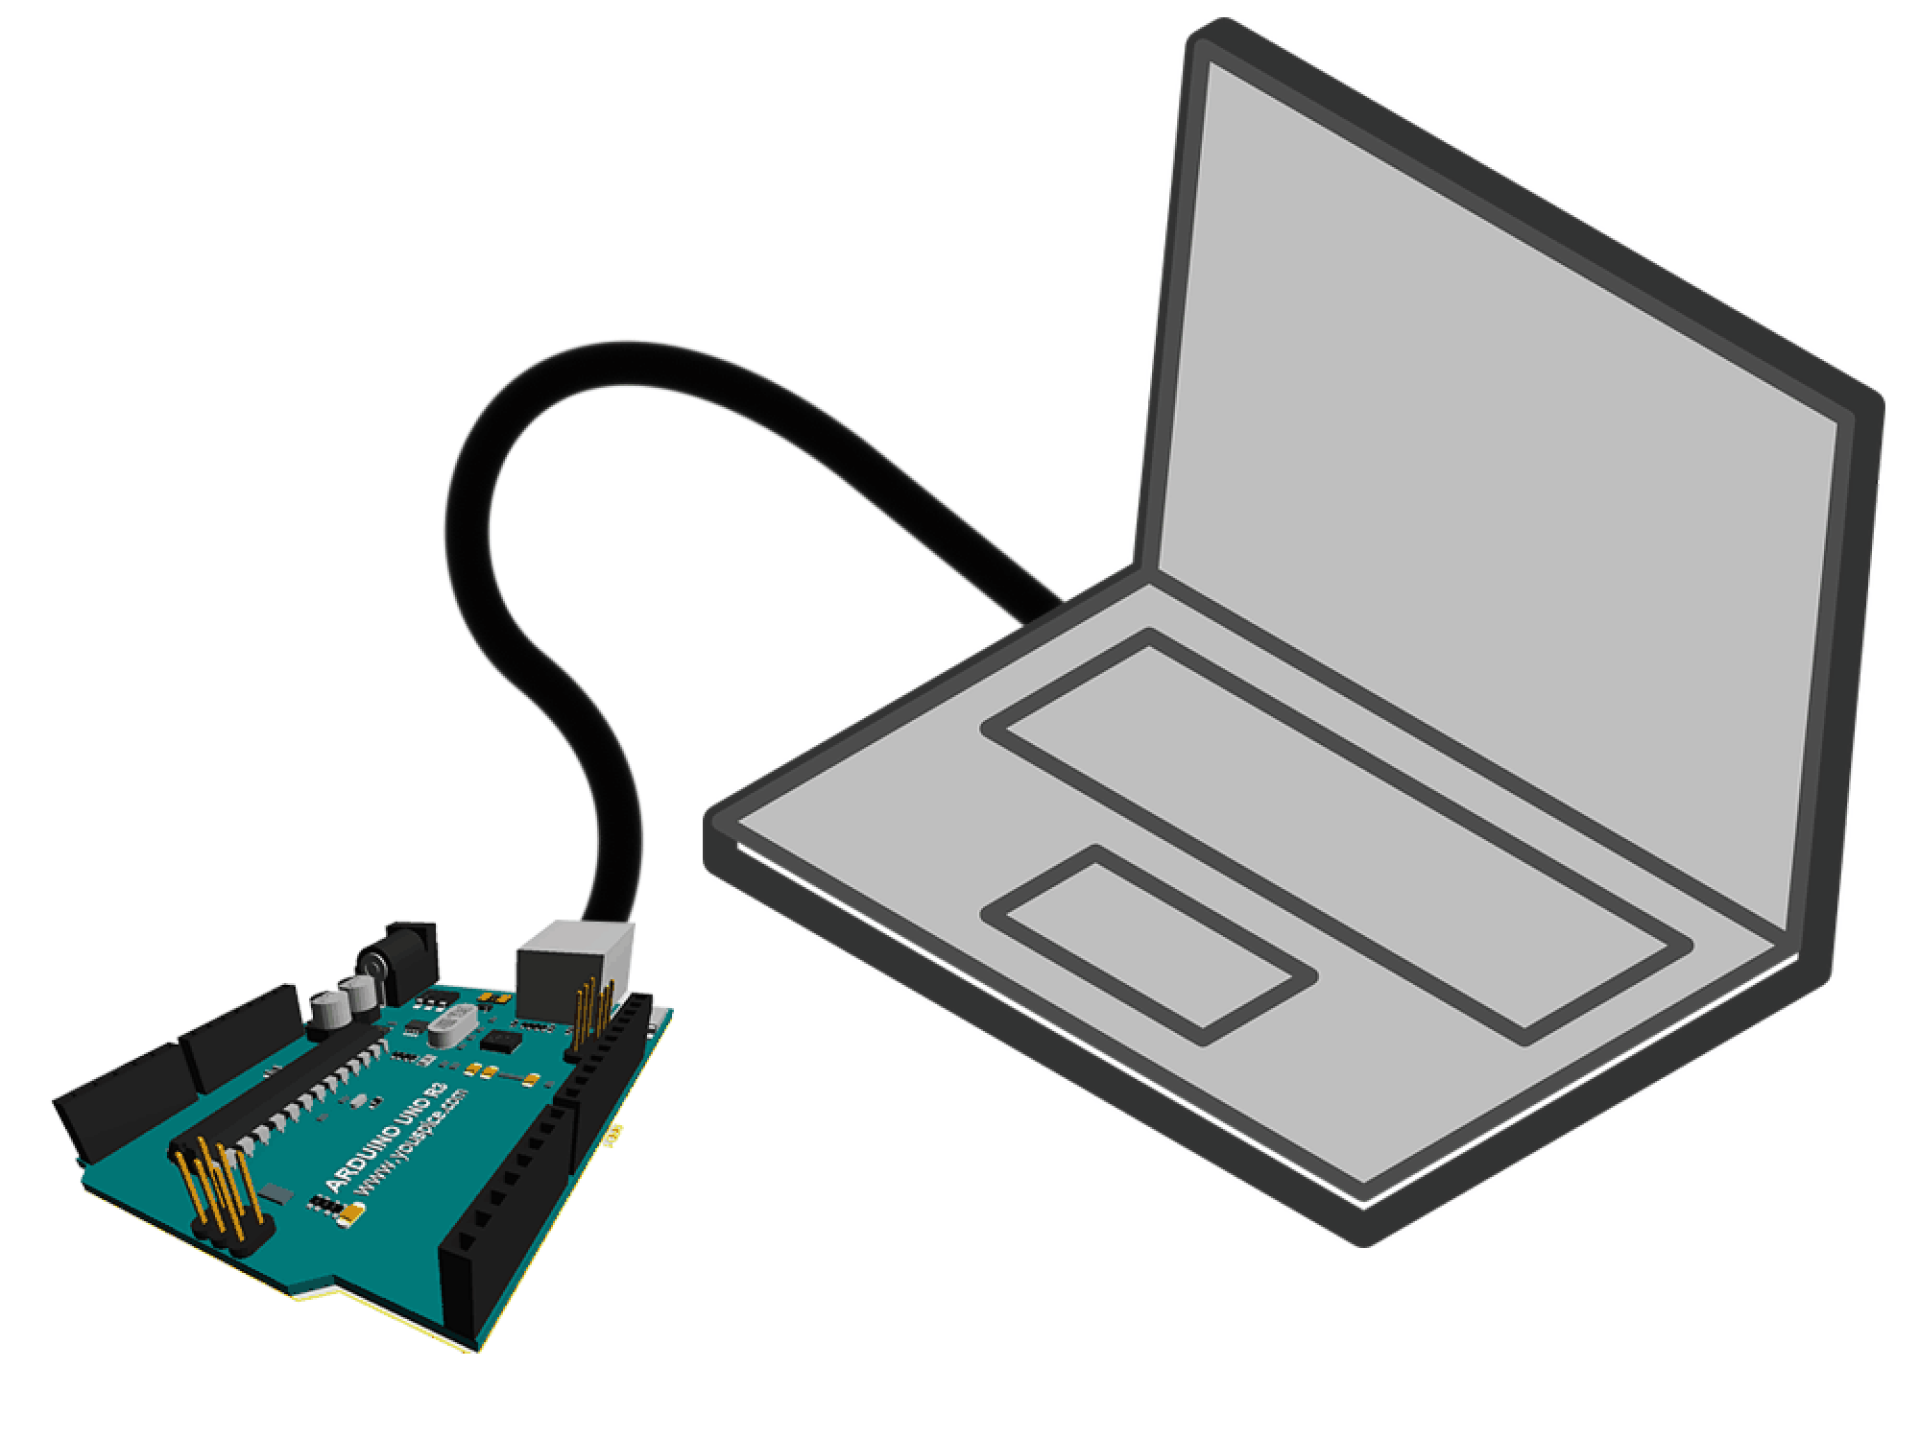
\includegraphics[width=0.8\linewidth]{P4/img/per1/step 1.png}
			\caption{Step 1}
			\label{fig:Step 1(Step 1)}
		\end{figure}
		\item Buka software Arduino IDE, lalu pilih new sketch.
		\begin{figure}[H]
			\centering
			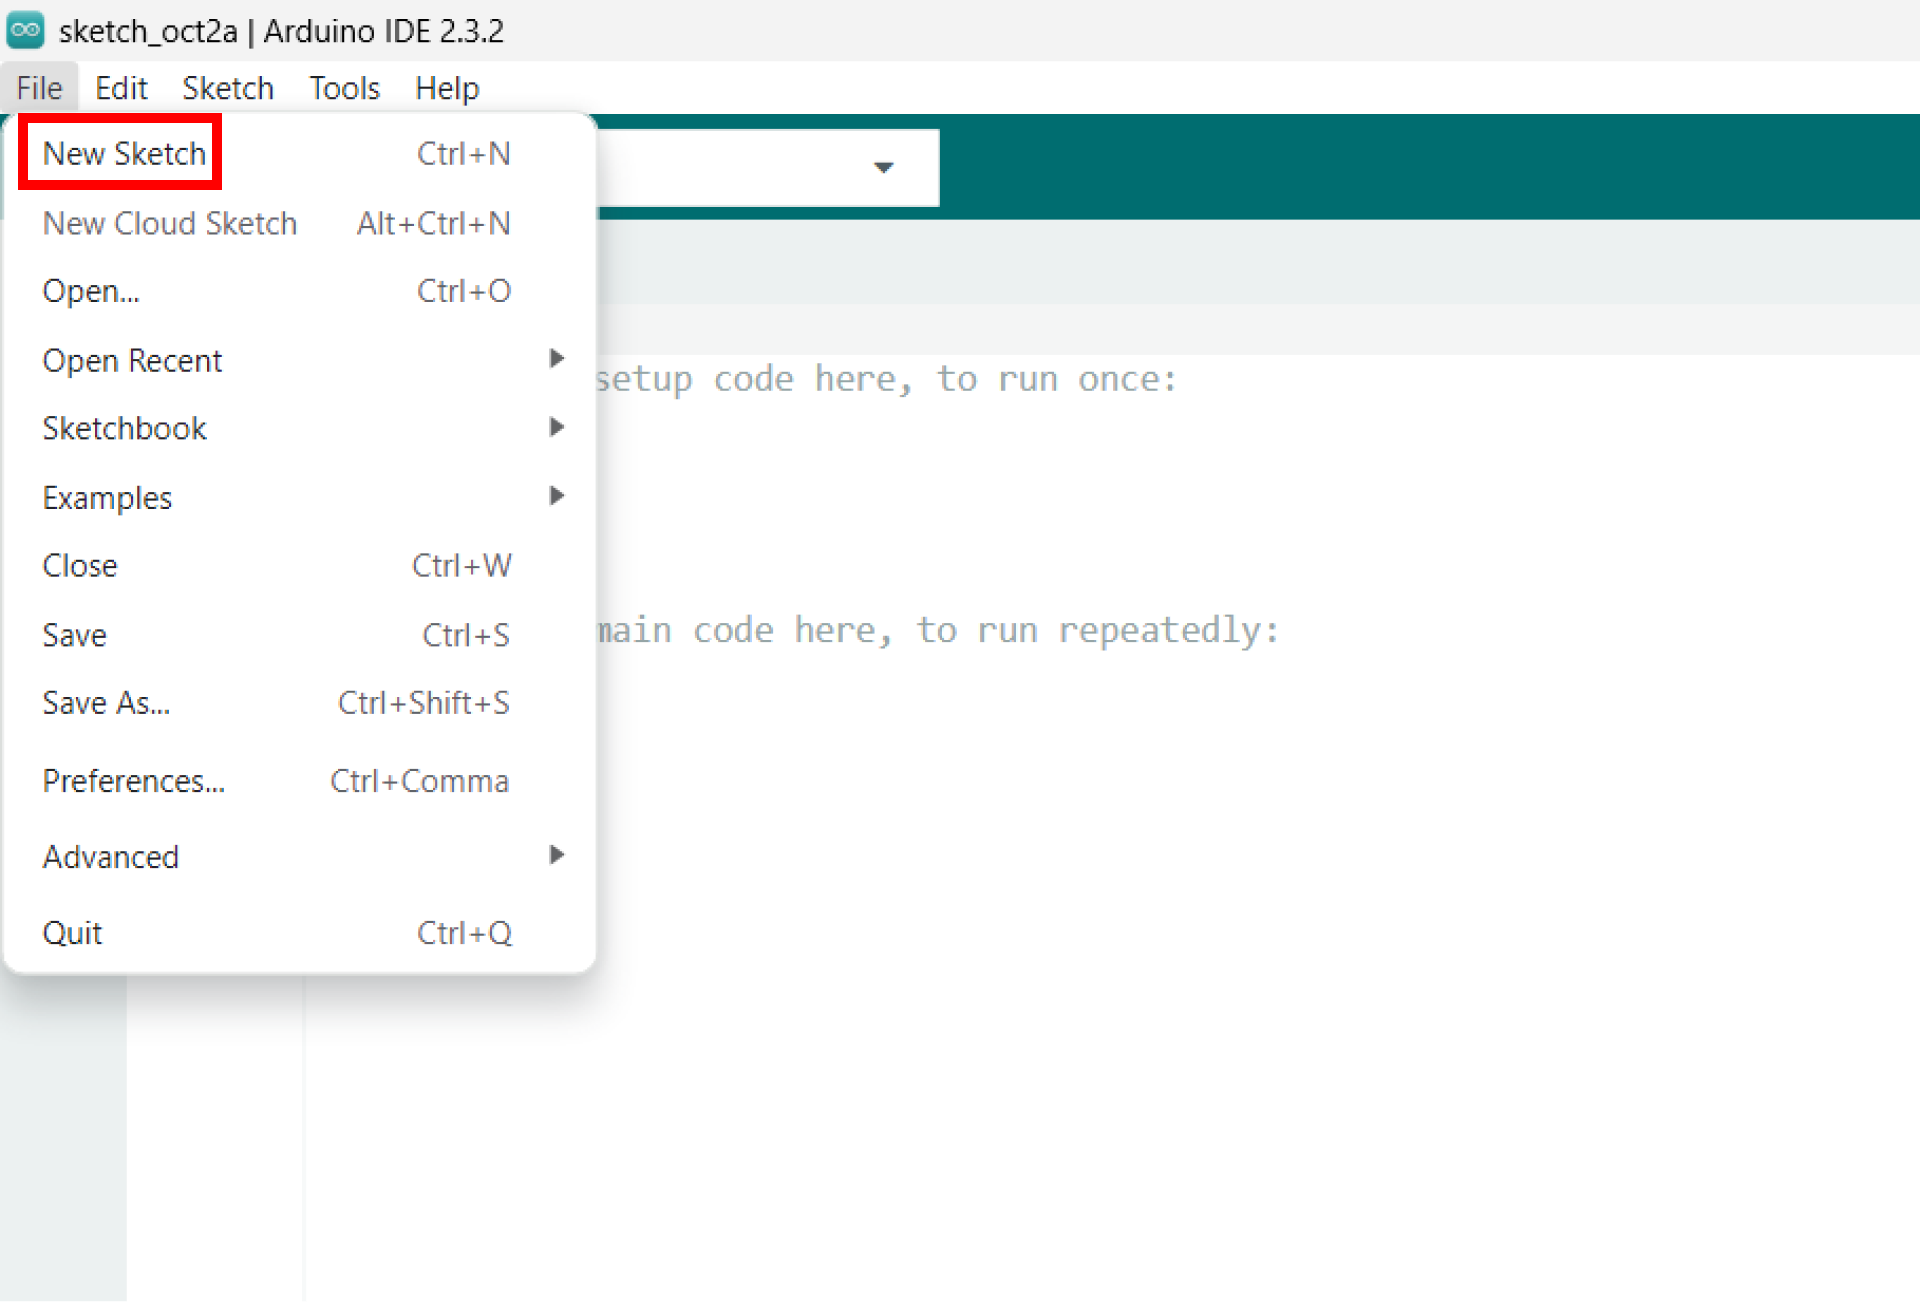
\includegraphics[width=0.8\linewidth]{P4/img/per1/step 2.png}
			\caption{Step 2}
			\label{fig:Step 2(Step 2)}
		\end{figure}
		\item Buka menu Tools, lalu cek Board dan Port yang terhubung apakah sudah benar
		\\(Port bergantung pada device, jadi bisa berbeda dengan port di Modul).
		\begin{figure}[H]
			\centering
			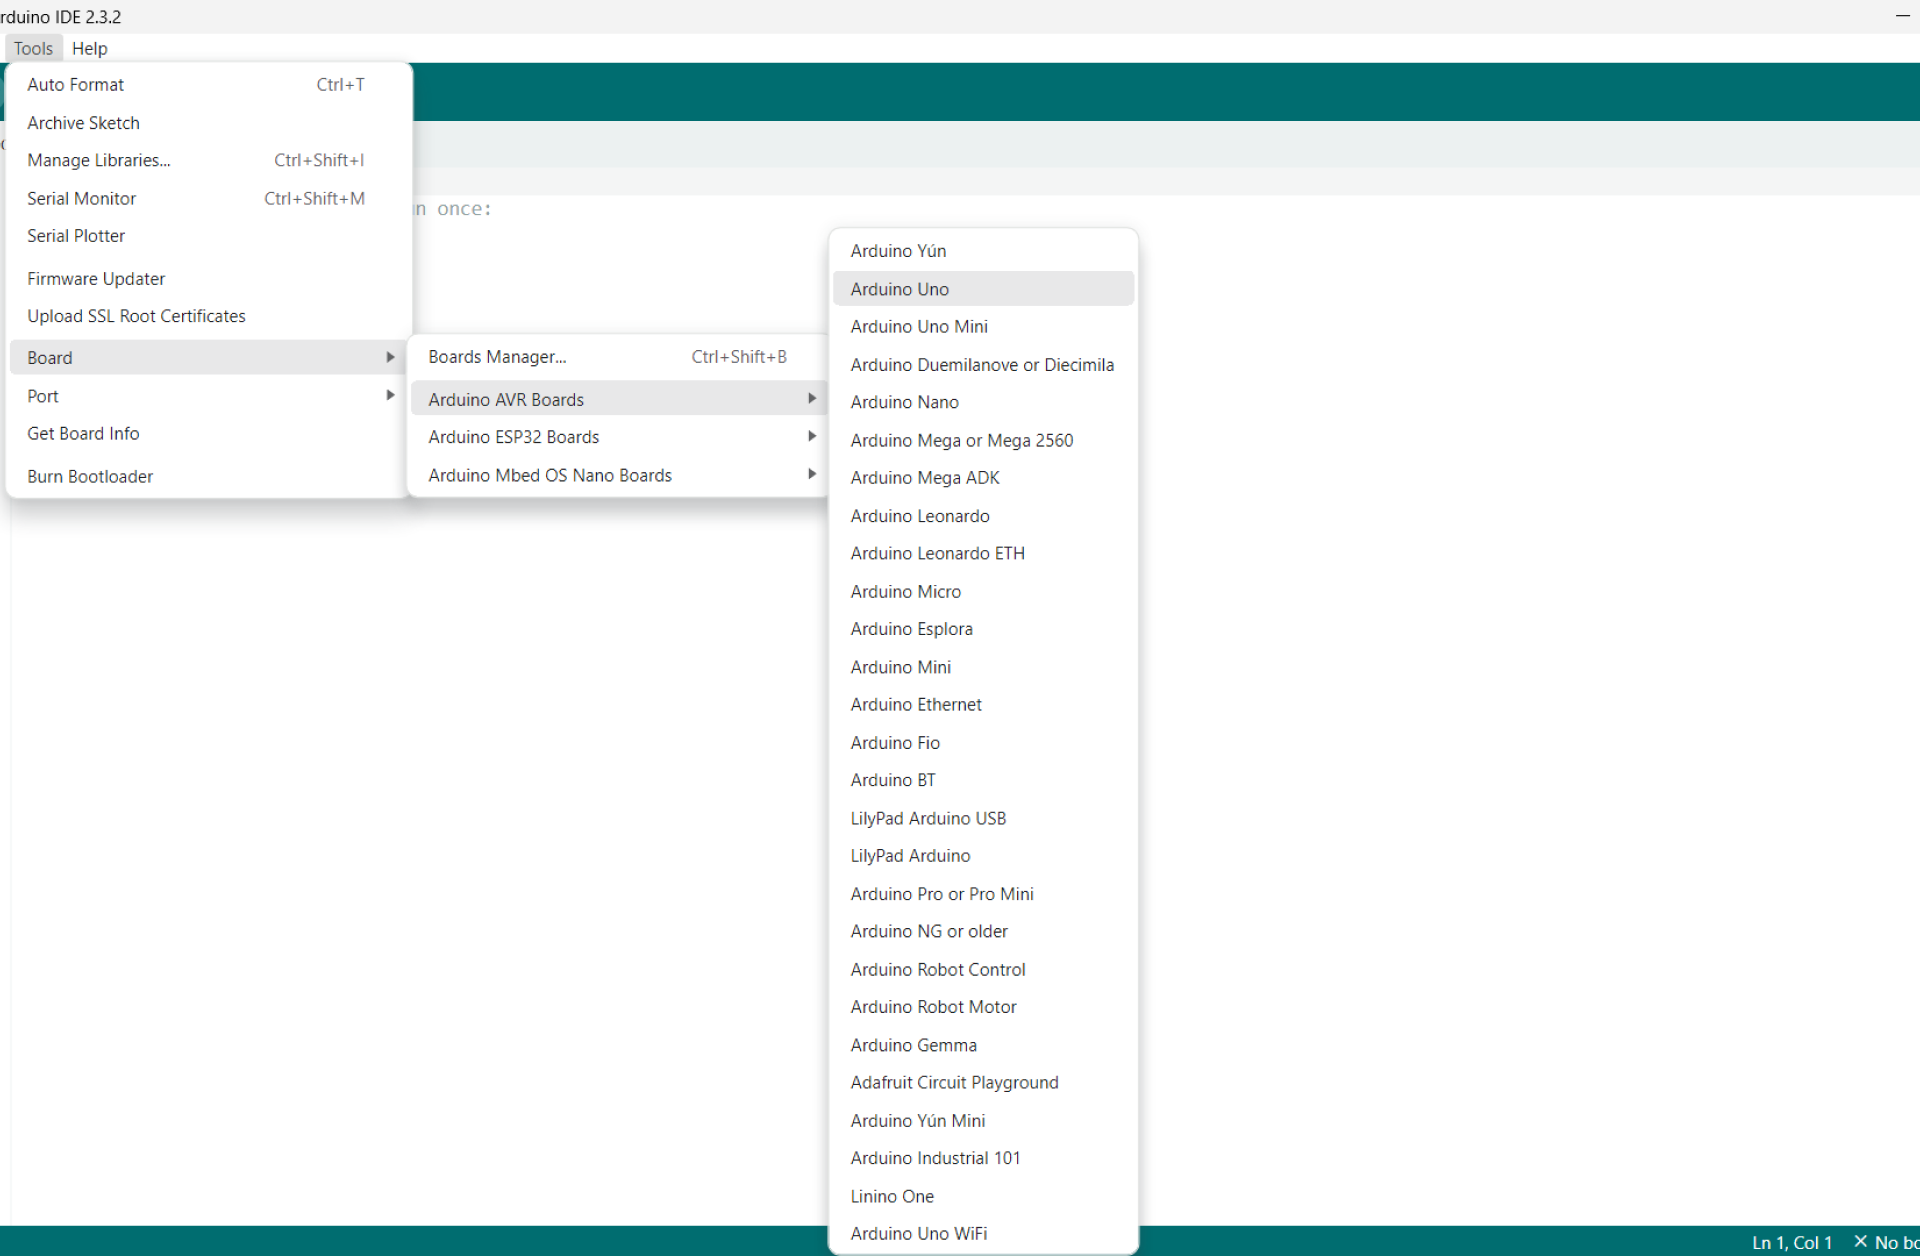
\includegraphics[width=0.8\linewidth]{P4/img/per1/step 3.png}
			\caption{Step 3}
			\label{fig:Step 3(Step 3)}
		\end{figure}
		\begin{figure}[H]
			\centering
			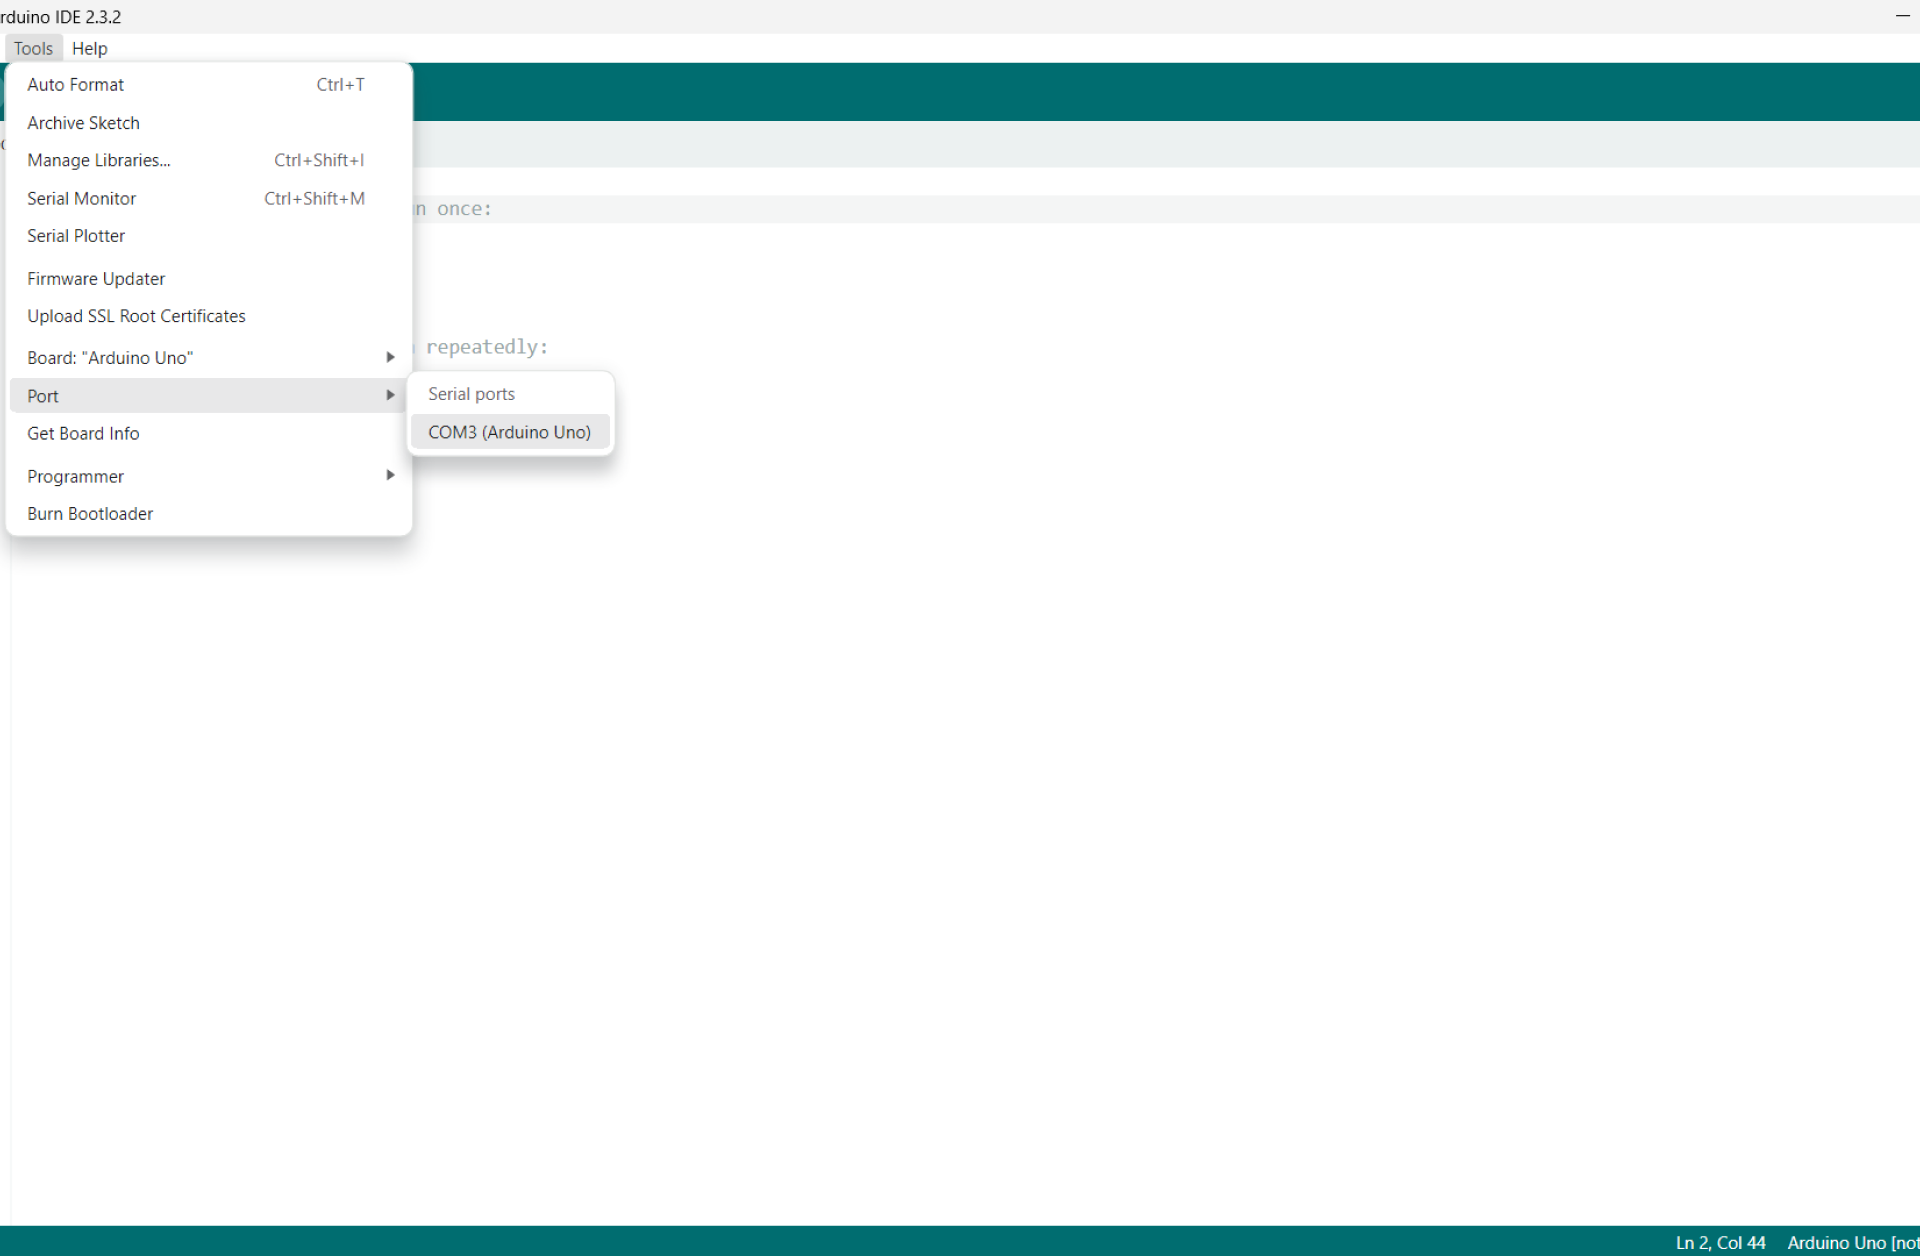
\includegraphics[width=0.8\linewidth]{P2/img/per1/step 4.png}
			\caption{Step 4}
			\label{fig:Step 4(Step 4)}
		\end{figure}
	
	\textbf{Kode Program Arduino}
		\item Masukkan kode program dibawah ini untuk menjalankan Digital Filter pada Arduino IDE.
		\begin{figure}[H]
			\centering
			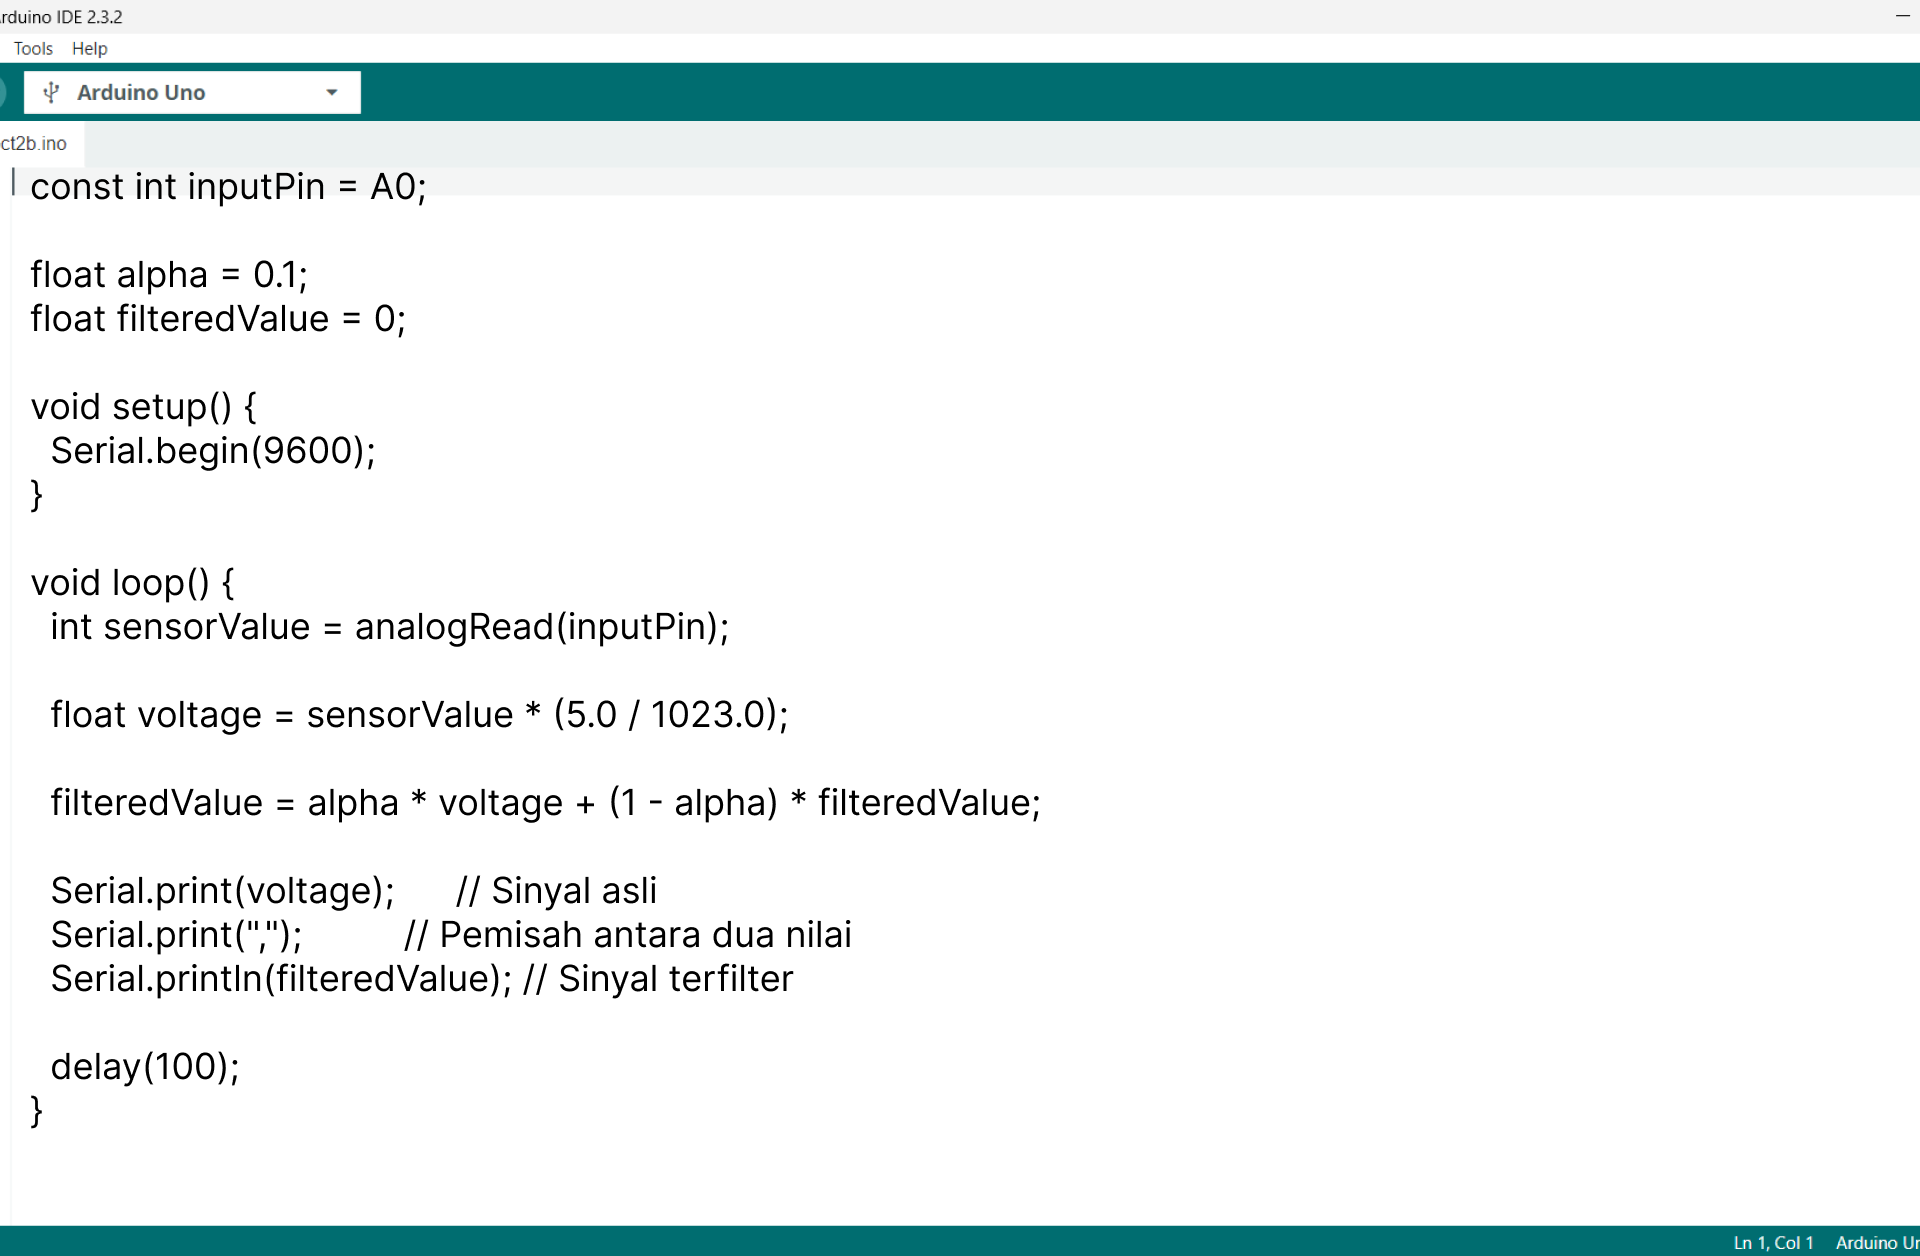
\includegraphics[width=0.8\linewidth]{P4/img/per1/step 5.png}
			\caption{Step 5}
			\label{fig:Step 5(Step 5)}
		\end{figure}
	
		\item Klik verify, apabila berhasil maka klik upload.
	\end{enumerate}
	
	\textbf{Memulai Function Generator}
	\begin{enumerate}
		\item Klik tombol power, untuk menyalakan function generator.
		\begin{figure}[H]
			\centering
			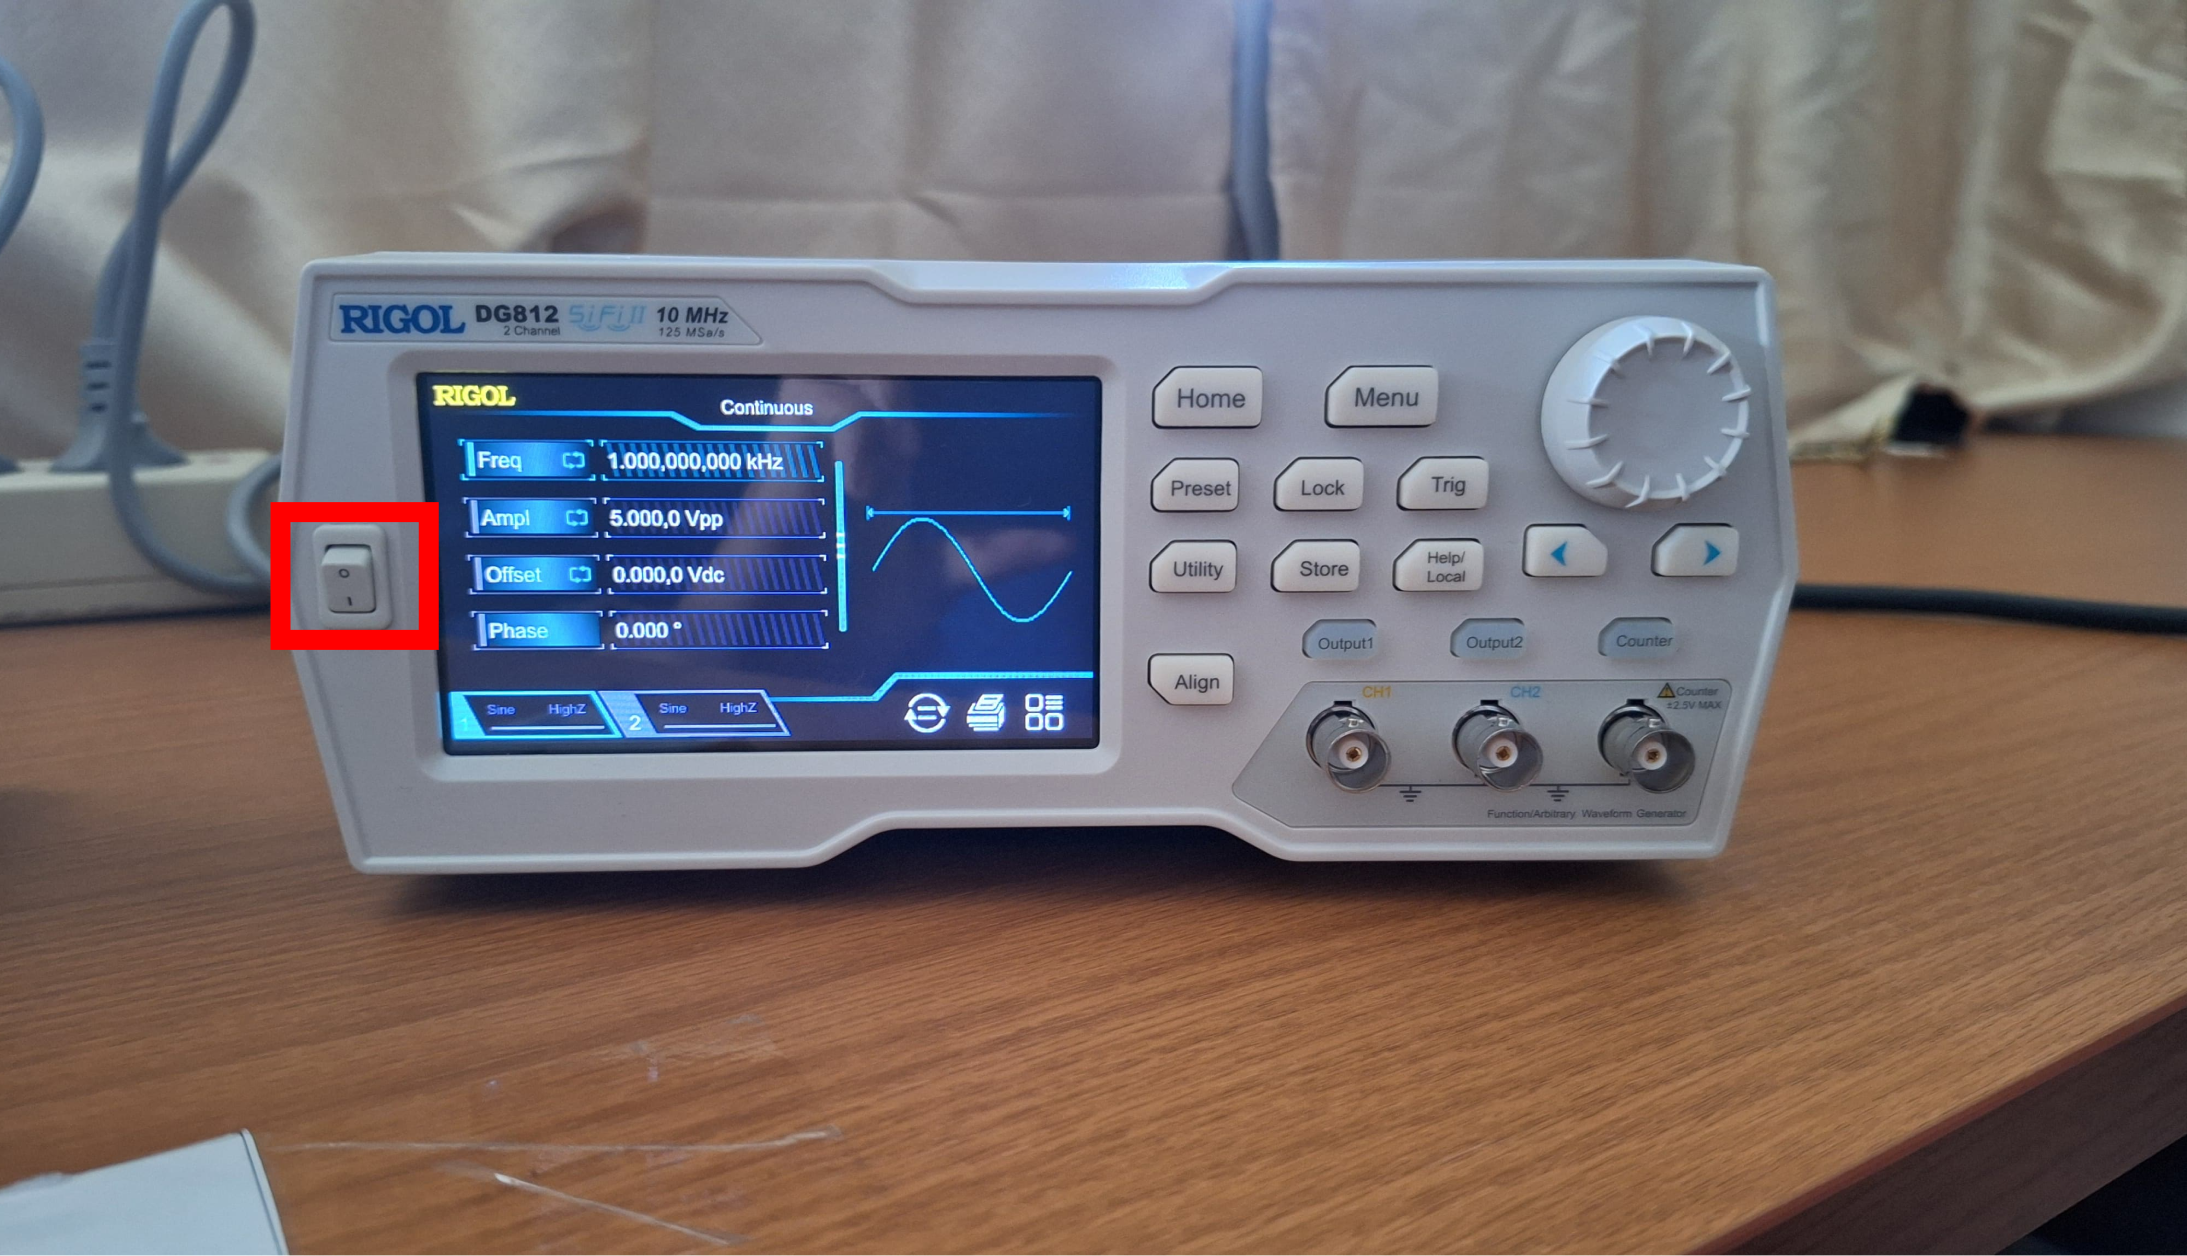
\includegraphics[width=0.8\linewidth]{P4/img/per1/step 6.png}
			\caption{Step 6}
			\label{fig:Step 6(Step 6)}
		\end{figure}

		\item Konfigurasi sinyal input pada Function generator.
		\begin{figure}[H]
			\centering
			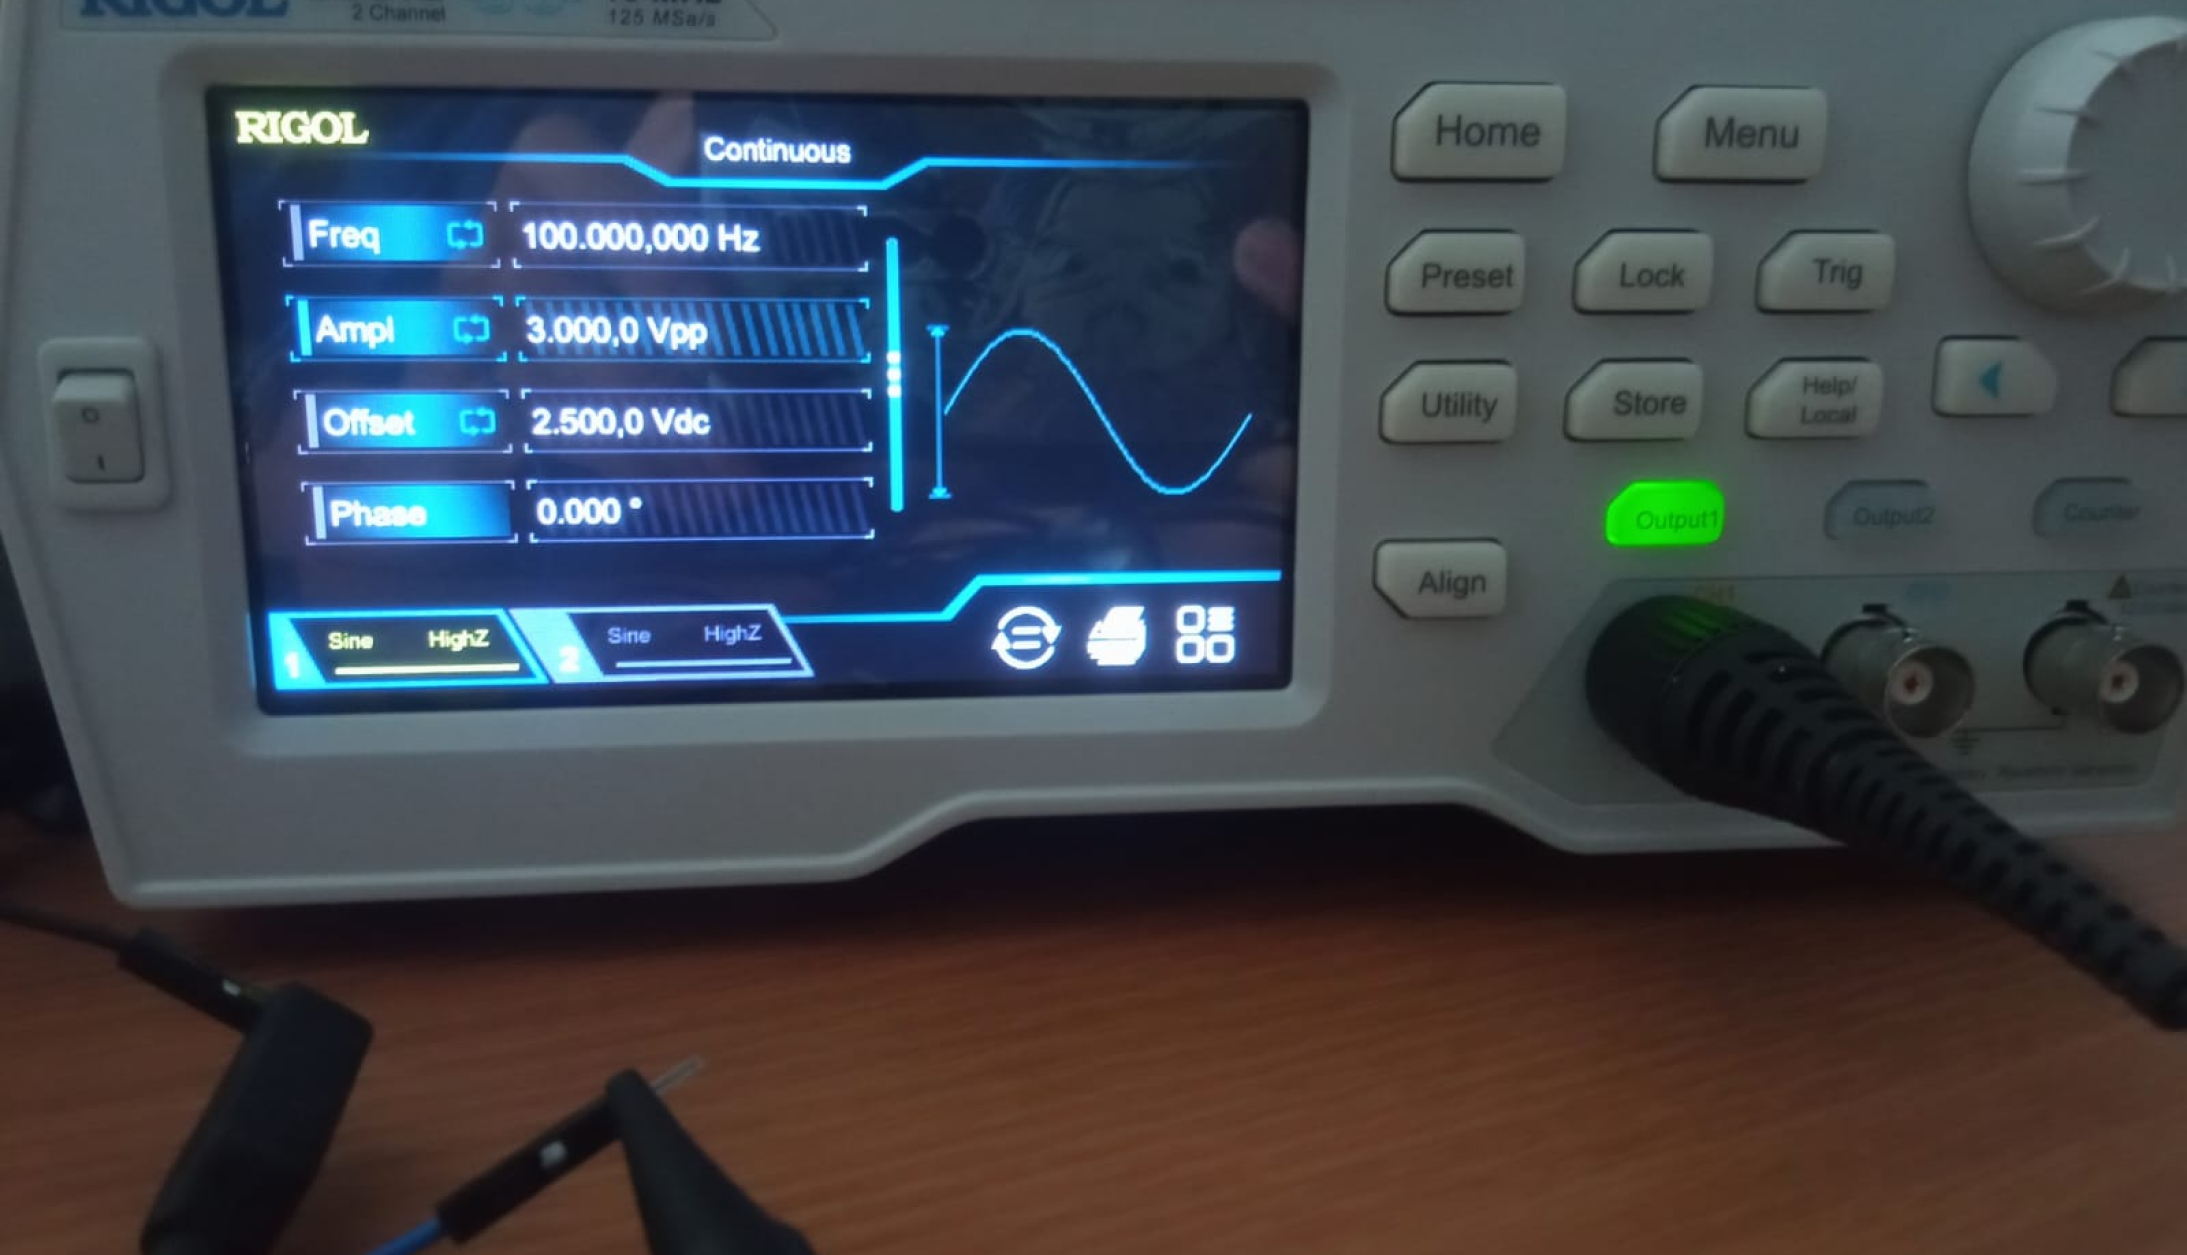
\includegraphics[width=0.8\linewidth]{P4/img/per1/step 7.png}
			\caption{Step 7}
			\label{fig:Step 7(Step 7)}
		\end{figure}
	\end{enumerate}

	\textbf{Konfigurasi Arduino}
	\begin{enumerate}
		\item Hubungkan kabel jumper ke salah satu pin Analog Arduino, kemudian hubungan ke probe.
		\\pengait (positif) Function generator.
		\begin{figure}[H]
			\centering
			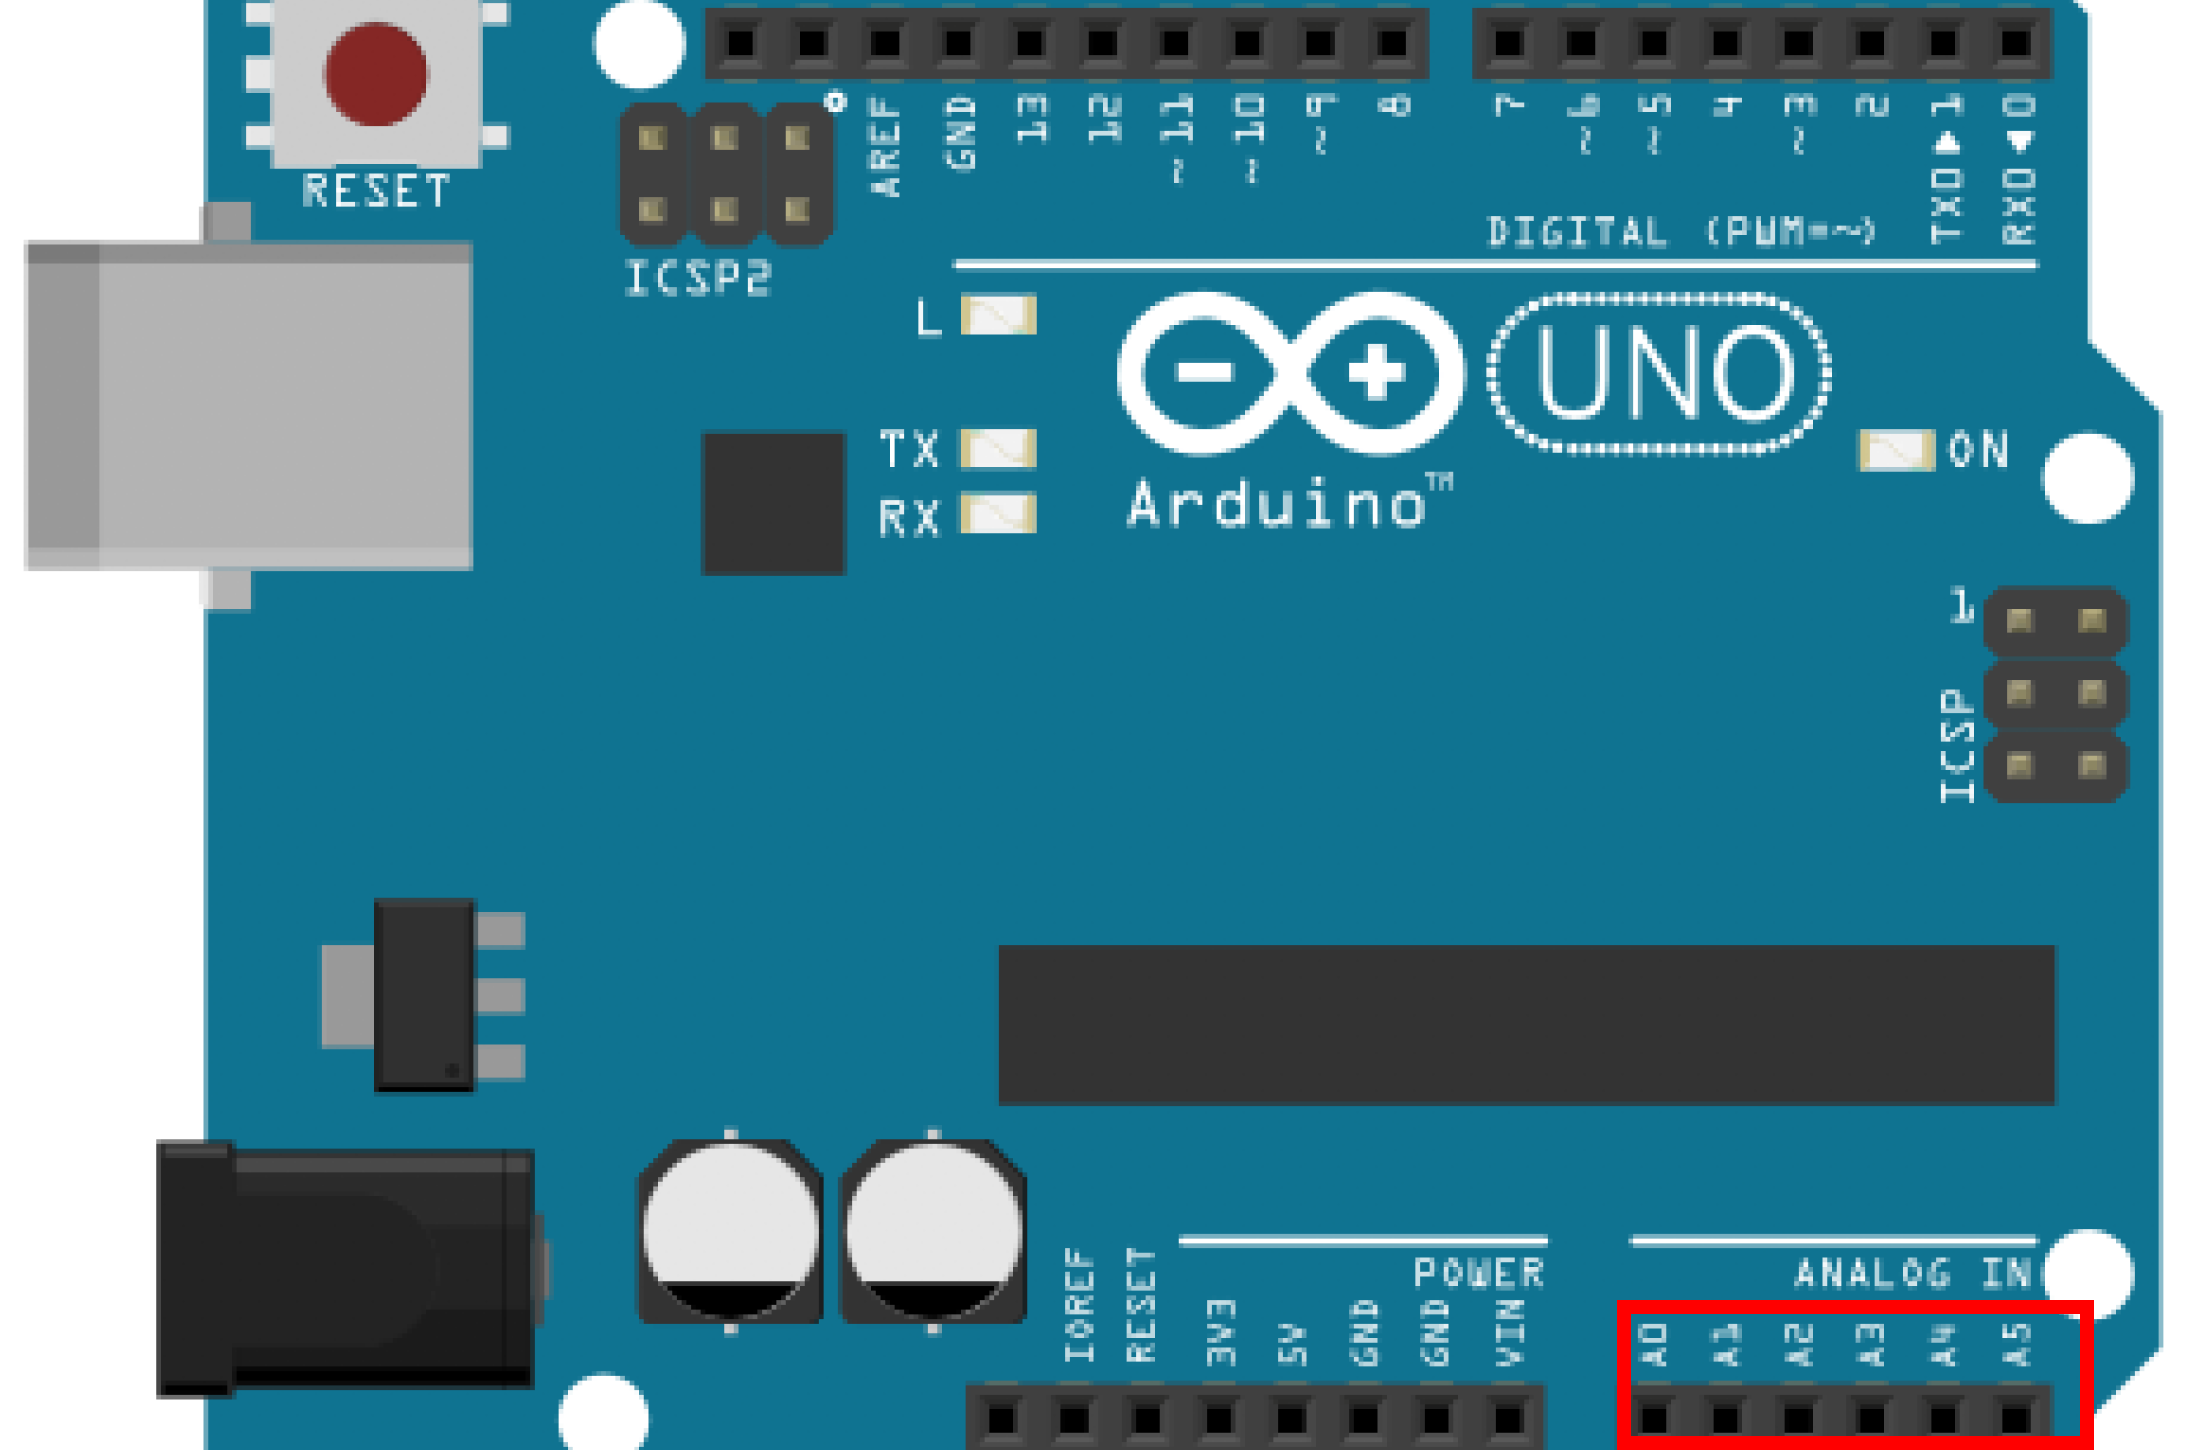
\includegraphics[width=0.8\linewidth]{P4/img/per1/step 8.png}
			\caption{Step 8}
			\label{fig:Step 8(Step 8)}
		\end{figure}

		\item Hubungkan kabel jumper ke salah satu pin GND Arduino, kemudian hubungkan probe.
		\\penjepit buaya (negatif) Function generator.
		\begin{figure}[H]
			\centering
			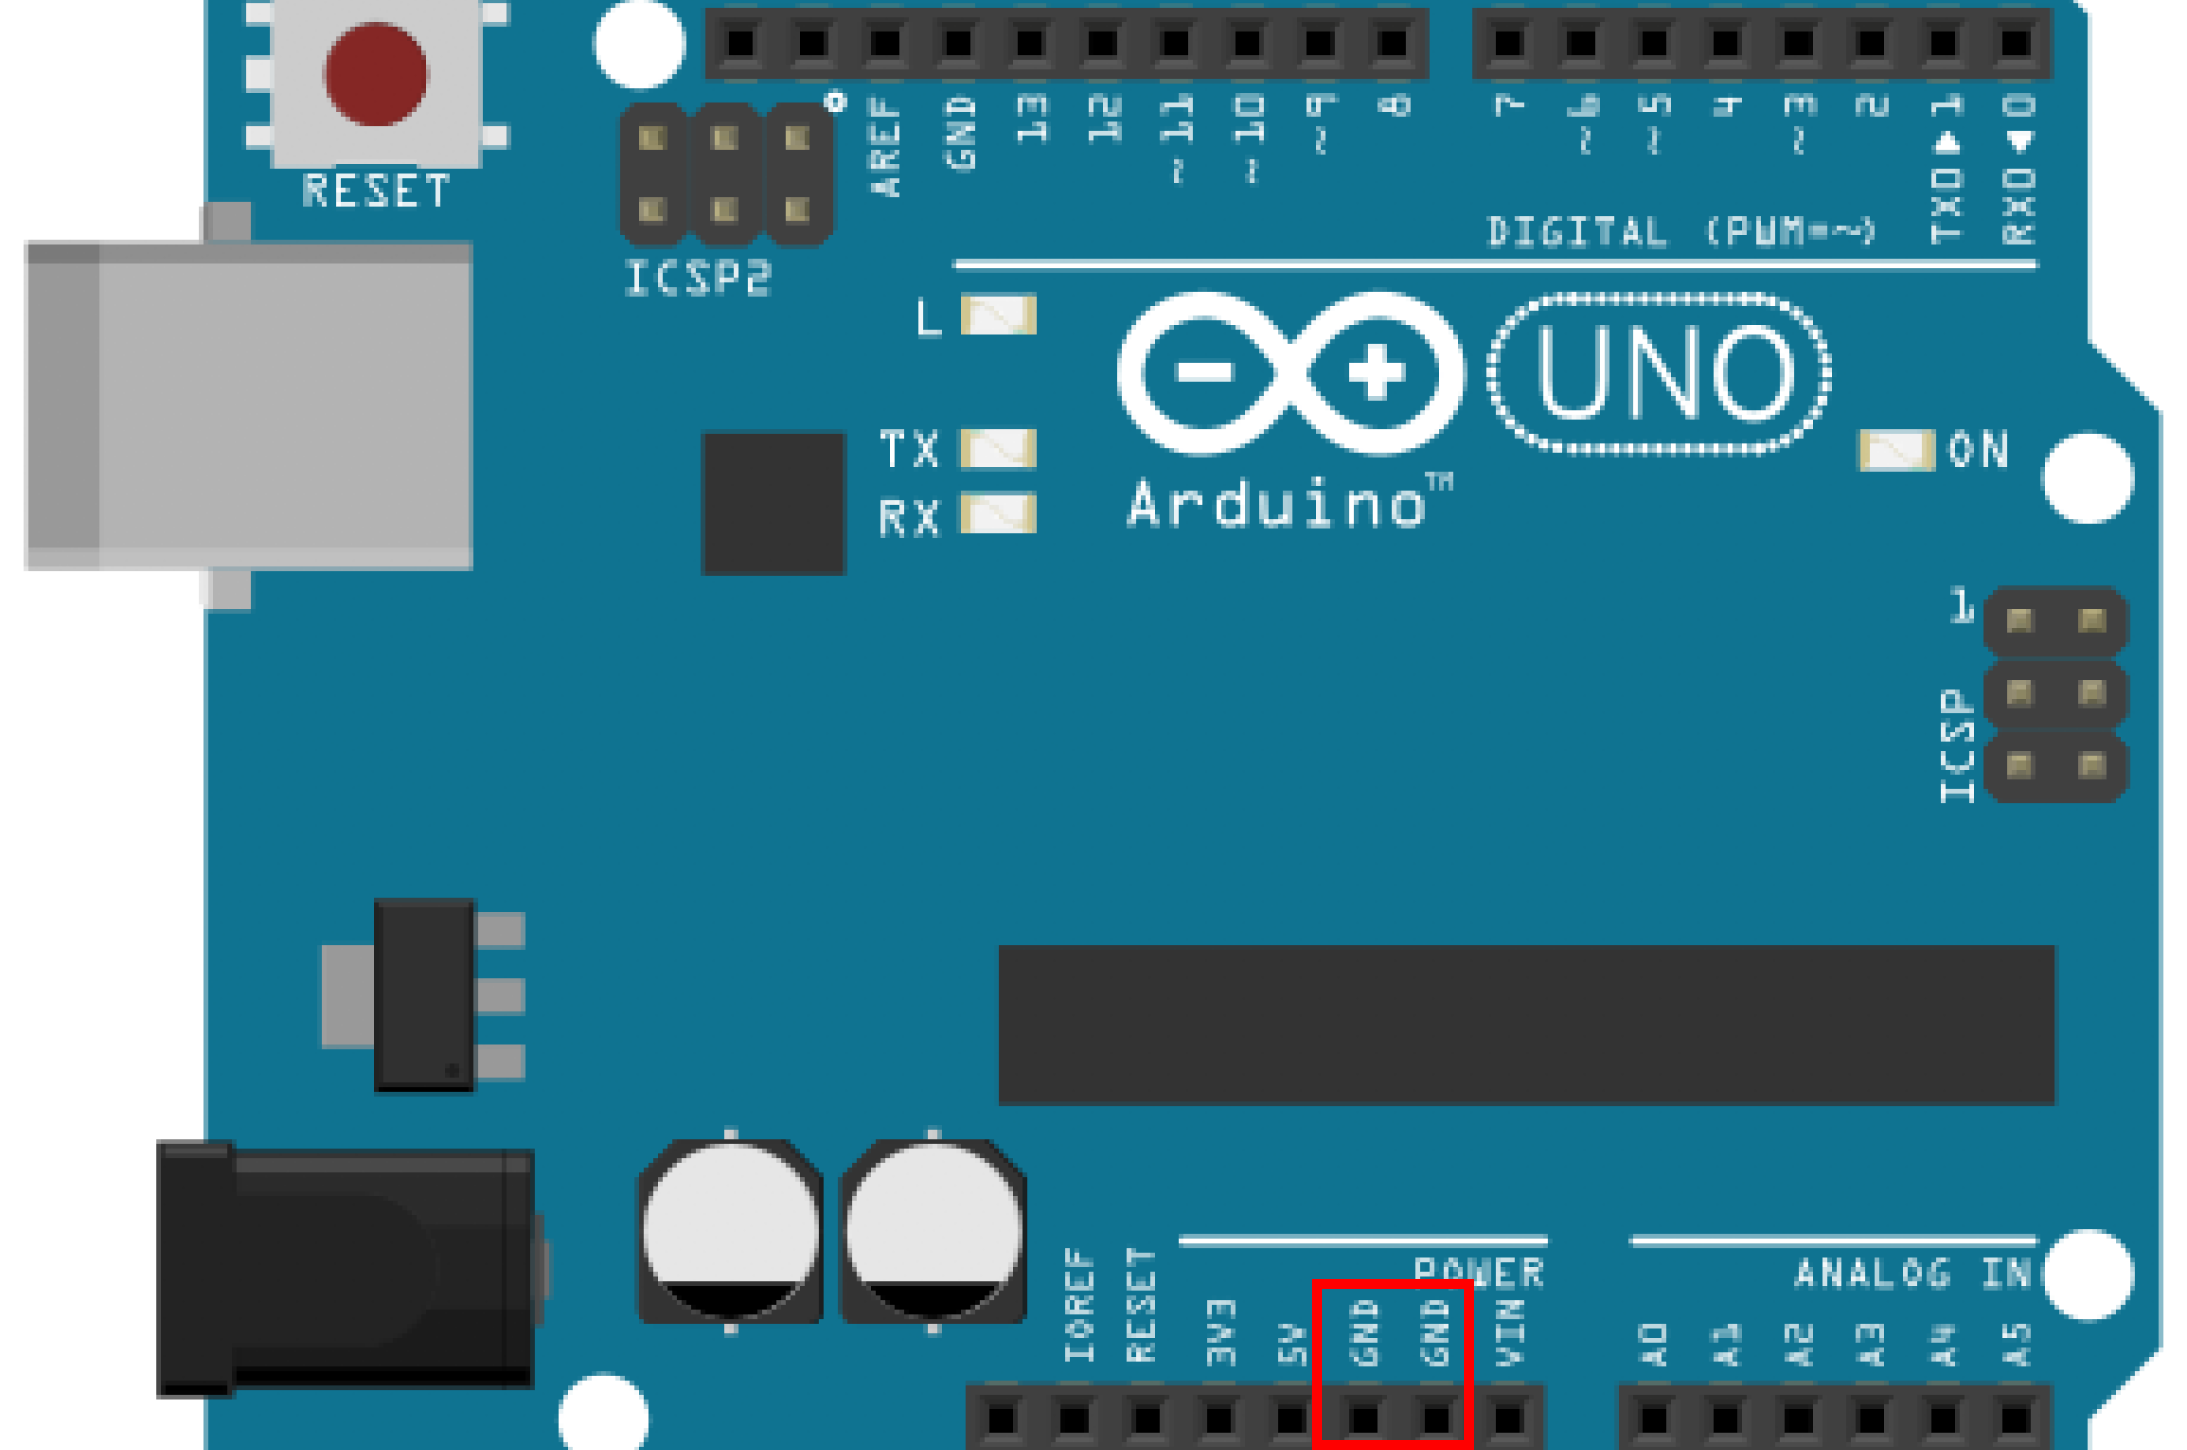
\includegraphics[width=0.8\linewidth]{P4/img/per1/step 9.png}
			\caption{Step 9}
			\label{fig:Step 9(Step 9)}
		\end{figure}

		\item Nyalakan Output 1 pada Function Generator.
		\item Buka Serial plotter di pojok kanan atas pada Arduino IDE.
		\item Buka Serial Monitor di pojok kanan atas pada Arduino IDE.
	\end{enumerate}

\end{center}

%======================PERCOBAAN 2==========================%
\subsection{Percobaan 2}
\begin{center}
	\textbf{Konfigurasi Osiloskop}
	\begin{enumerate}
		\item Hubungkan kabel power ke osiloskop, lalu tekan tombol power untuk menyalakan Osiloskop. 
		\begin{figure}[H]
			\centering
			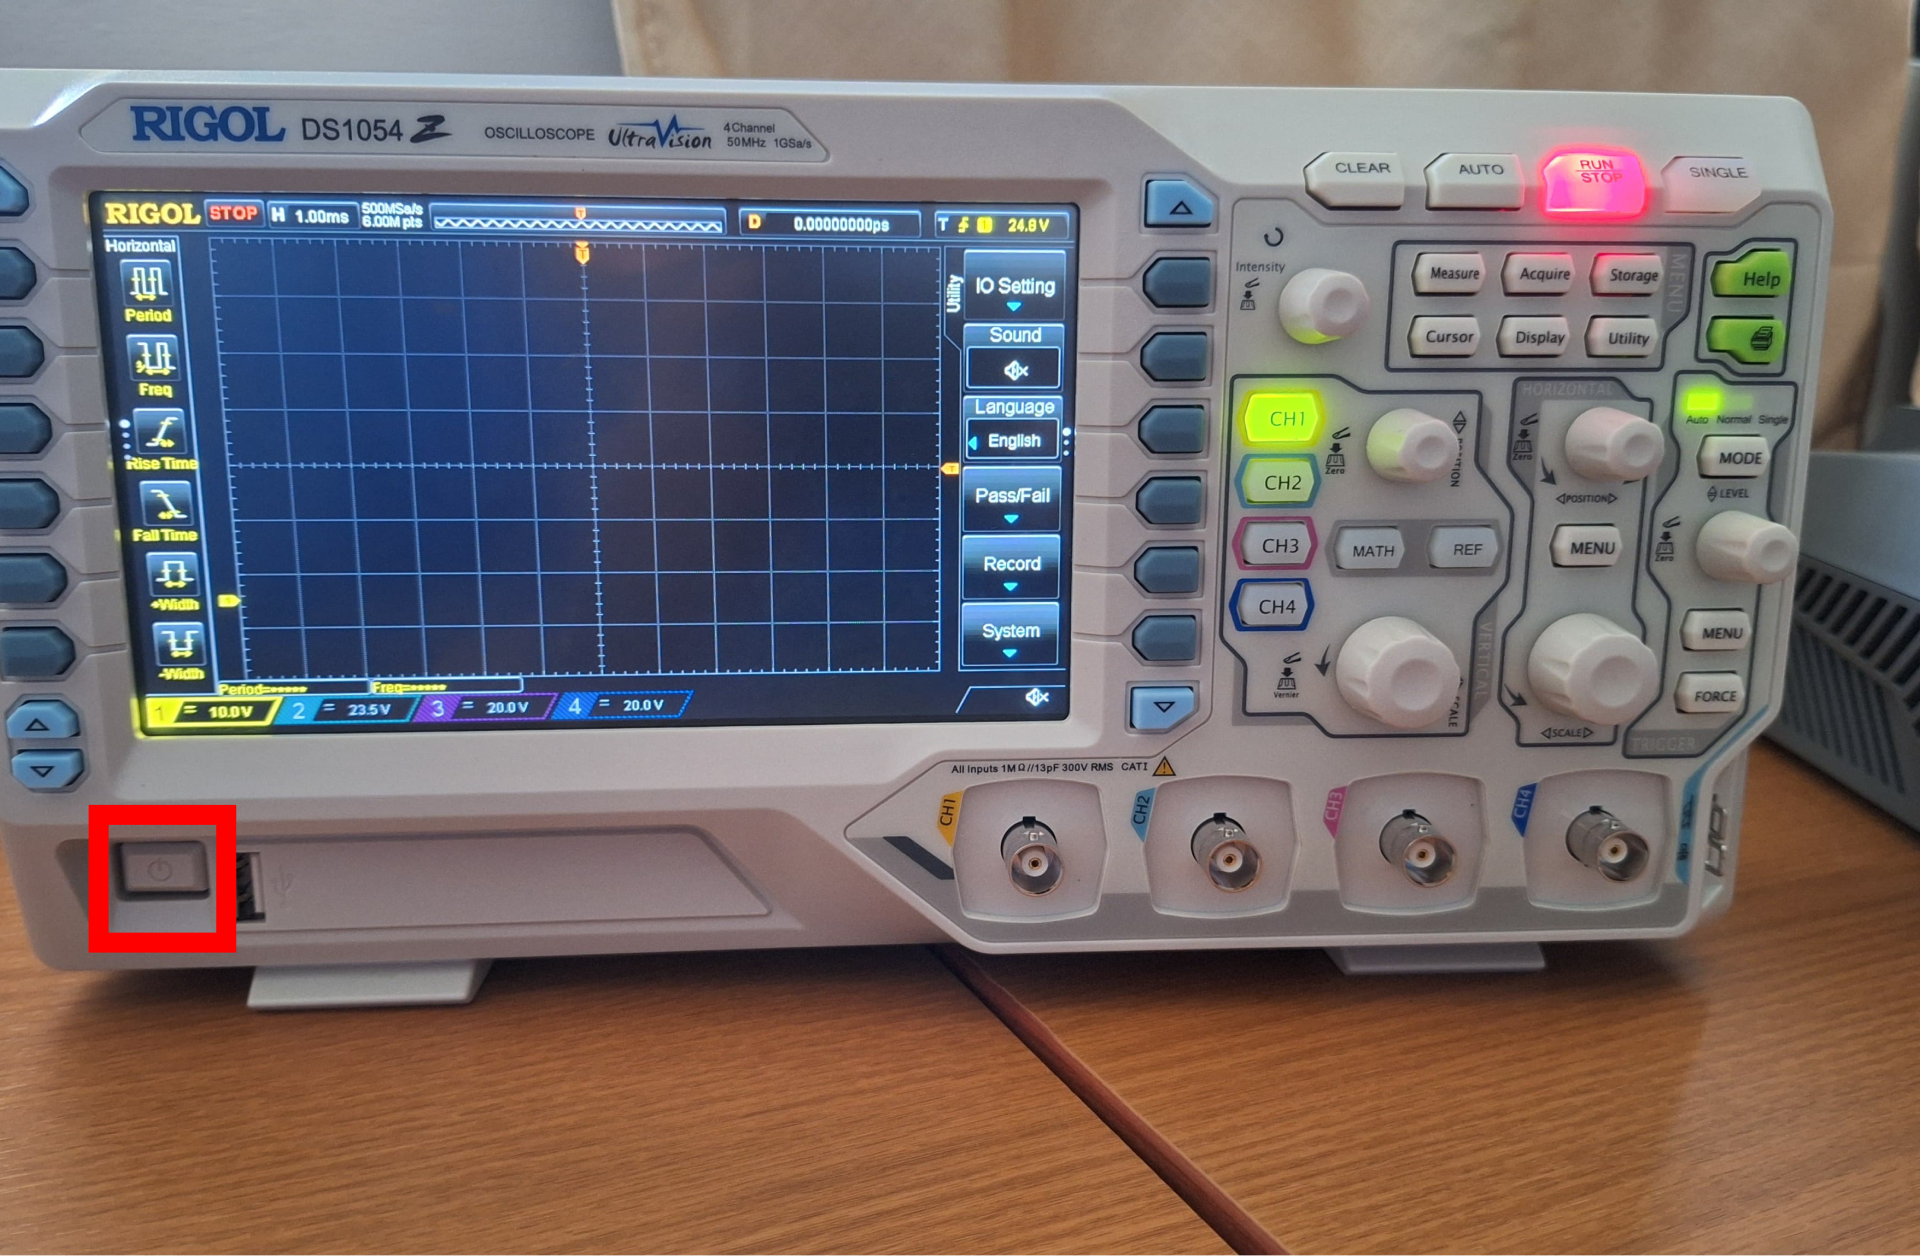
\includegraphics[width=0.9\linewidth]{P4/img/per2/step 1.png}
			\caption{Step 1}
			\label{fig:Step 1(Step 1)}
		\end{figure}

		\item Hubungkan kabel probe pada channel 1. 
		\begin{figure}[H]
			\centering
			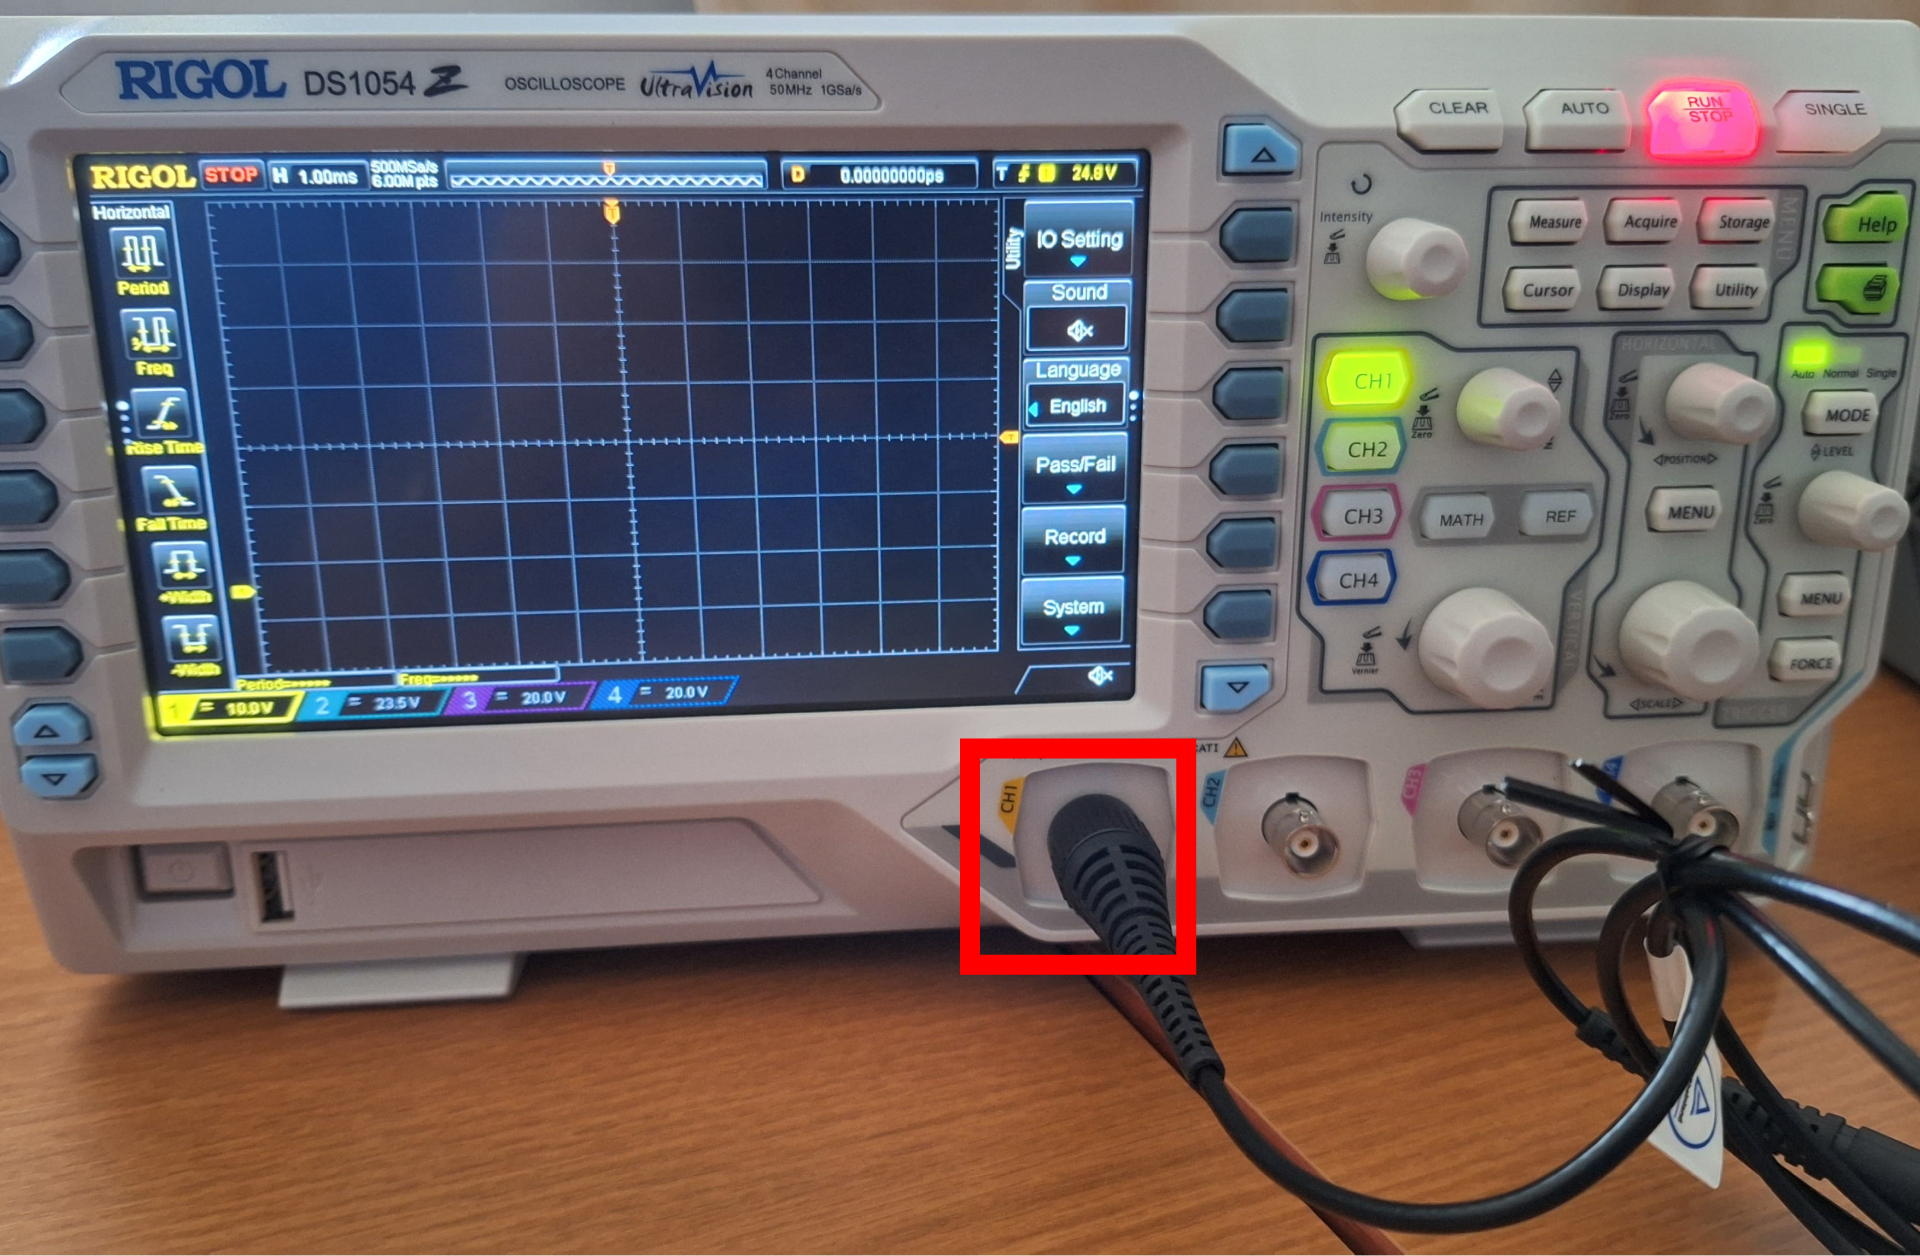
\includegraphics[width=0.8\linewidth]{P4/img/per2/step 2.png}
			\caption{Step 2}
			\label{fig:Step 2(Step 2)}
		\end{figure}

		\item Hubungkan kabel jumper dari salah satu pin Analog Arduino dengan probe pengait (positif) osiloskop dan function generator.
		\item Hubungkan kabel jumper pin GND Arduino dengan probe penjepit buaya (negatif) osiloskop.
		\item Klik AUTO pada Osiloskop.
		\item Bandingkan hasil sinyal yang ditampilkan oleh Serial plotter Arduino dengan Osiloskop.
	\end{enumerate}	
\end{center}

%===========================================================%
\section{Hasil yang didapat}
Memahami perbedaan hasil sinyal digital yang diperoleh oleh Arduino dan Osiloskop.

%===========================================================%
\section{Kesimpulan}
Mengetahui hasil sinyal manakah yang lebih baik dihasilkan dari kedua perangkat \\Arduino dan Osiloskop.
